\chapter{\IfLanguageName{dutch}{proof-of-concept}{proof-of-concept}}%
\label{ch:proof-of-concept}
\section{Inleiding}
In dit hoofdstuk bespreken we de implementatie van het proof-of-concept. We bespreken elke fase van het proces in detail en zullen de implementatie van de bijbehorende componenten toelichten. Hierbij gaan we ook de uitkomsten van elke fase beschrijven en hoe deze  gebruikt kunnen worden in de volgende fase. 

\section{Webscraper}
\subsection{Algemene Eisen}
Binnen de algemene eisen zal de webscraper voldoen aan de ethische aspecten beschreven in sectie \ref{subsection:scraper-ethische-aspecten}. Dit betekent dat de scraper de regels en richtlijnen van de gescrapte websites zal respecteren en zich zal houden aan eventuele beperkingen zoals vermeld in het robots.txt-bestand. Hierdoor wordt ervoor gezorgd dat de scrapingactiviteiten op een ethisch verantwoorde manier worden uitgevoerd. \\

Daarnaast zal de webscraper in staat zijn om verschillende websites te scrapen, met de focus op het verzamelen van de frontpage-inhoud. Specifiek zal de scraper de eerste 20 items van de frontpage van elke website verzamelen. \\

De webscraper zal twee bekende nieuwsbronnen scrapen, namelijk HLN en DeMorgen.

\subsection{Verkenning}
Alvorens we de webscraper kunnen implementeren, is het nodig om de DOM-structuur \footnote{De DOM-structuur (Document Object Model) is een hiërarchische representatie van een HTML- of XML-document.} van beide websites te bekijken en een patroon hierin te herkennen. 
\subsubsection{HLN}
Op de startpagina van HLN kunnen we zien in figuur \ref{fig:hln_frontpage} dat elk nieuwsartikel zich bevindt binnen een article-tag bevindt. De eerste subtag is een a-tag met hierin de href naar het artikel. \\ 

Deze href zal belangrijk zijn om de datum te valideren en de titel te extraheren. We moeten deze dus opslaan. 

\begin{center}
    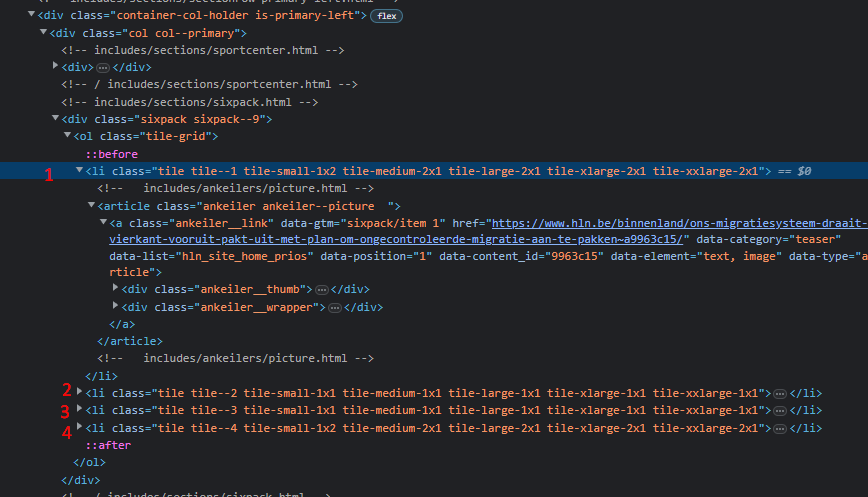
\includegraphics[width = 6in]{hln_frontpage2.png}
    \captionof{figure}{DOM-structuur van de startpagina van HLN met hierop verschillende nieuwsartikels op aangeduid.}
    \label{fig:hln_frontpage}
\end{center}

Als we vervolgens gaan kijken naar de DOM-structuur van een artikel, zien we dat de titel weergegeven wordt binnen een header-tag met als class 'article\_\_header' deze titel heeft als class 'article\_\_title'. De datum wordt weergegeven binnen een time-tag met datetime als value en class 'article\_\_time'. De datum is ook opgemaakt in een bepaald formaat, dd-mm-yy, hh:mm. Deze gegevens zijn essentieel voor de scraper. In figuur \ref{fig:hln_article} vind je dit terug. \\

\begin{center}
    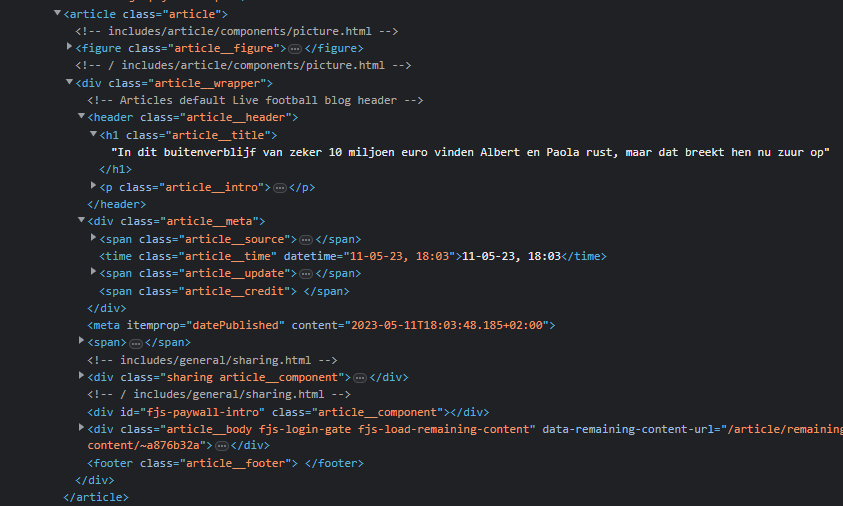
\includegraphics[width = 6in]{hln_article1.png}
    \captionof{figure}{DOM van een artikel op HLN.}
    \label{fig:hln_article}
\end{center}

\subsubsection{De Morgen}
De structuur van de artikels op de startpagina van De Morgen is vergelijkbaar met die van HLN. Zoals te zien is in figuur \ref{fig:demorgen_frontpage}, worden de artikels ook weergegeven binnen een article-tag, alleen is bij de morgen de tweede child de a-tag ten opzichte van HLN.

\begin{center}
    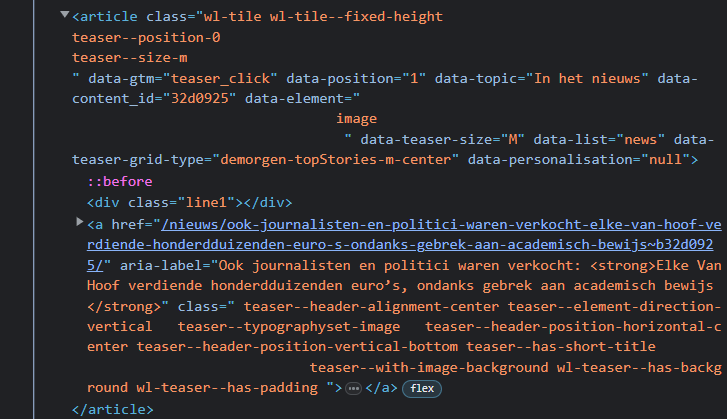
\includegraphics[width = 6in]{demorgen_frontpage2.png}
    \captionof{figure}{DOM van een artikel op De Morgen.}
    \label{fig:demorgen_frontpage}
\end{center}

Bij het doorklikken op een willekeurig artikel zien we dat de DOM-structuur vergelijkbaar is, maar niet exact hetzelfde qua structuur. In figuur \ref{fig:demorgen_article} zie je de DOM.

\begin{center}
    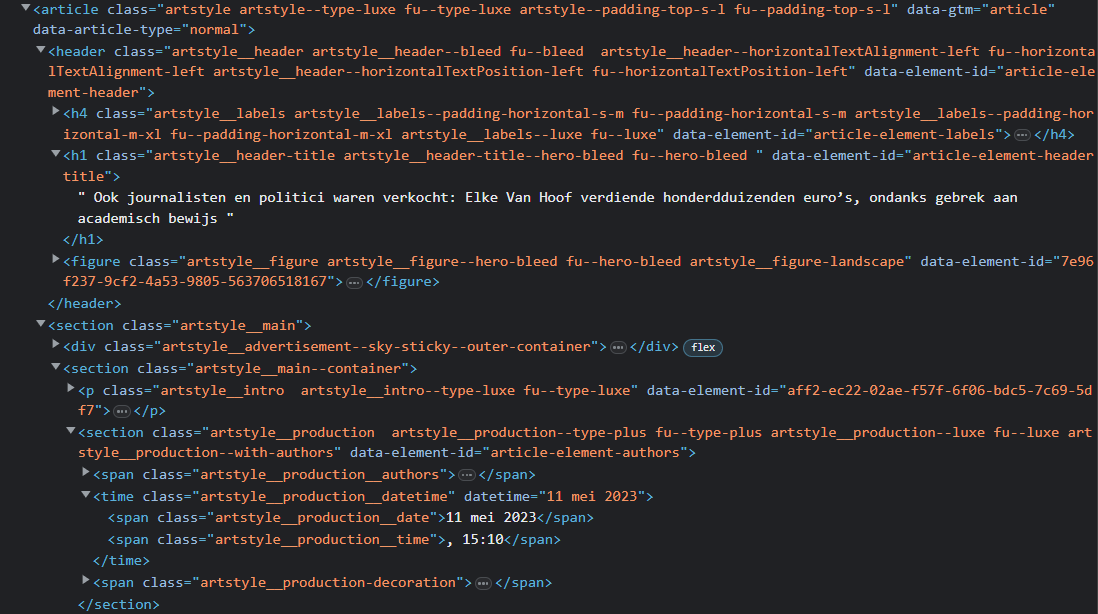
\includegraphics[width = 6in]{demorgen_article.png}
    \captionof{figure}{DOM van een artikel op De Morgen.}
    \label{fig:demorgen_article} 
\end{center}

Nu dat we deze informatie hebben. Kunnen we beginnen aan de implementatie van de scraper. 

\subsection{Implementatie}
\subsubsection{Thread-safe Dictionary}
Om ervoor te zorgen dat de gescrapete data veilig wordt opgeslagen, beginnen we de implementatie met het maken van een thread-safe dictionary.
\begin{pythoncode}{../../../workspace/paper/scraper/util/volatileDictionary.py}
Deze thread-safe dictionary zal de opslag van de gescrapete data beheren en ervoor zorgen dat er geen problemen ontstaan tijdens het wegschrijven van de gescrapete data.
\end{pythoncode}

\subsubsection{Abstracte Thread}
Voordat we de specifieke threads implementeren, maken we eerst een AbstractThread-klasse die de methoden definieert die door de specifieke threads zullen worden gebruikt.

De AbstractThread-klasse bevat het volgende:

\begin{itemize}
    \item \textbf{Constructor}: Initialiseert de gemeenschappelijke eigenschappen die vereist zijn door de specifieke threads.
    \item \textbf{Methoden}: Definieert de gemeenschappelijke methoden die door de specifieke threads zullen worden gebruikt.
\end{itemize}

Laten we de \textbf{constructor} van de AbstractThread-klasse bespreken:

\begin{pythoncode}{../../../workspace/paper/abstractThreadCTR.py}
    In de constructor initialiseren we de gemeenschappelijke eigenschappen die vereist zijn door de specifieke threads. Deze eigenschappen omvatten:
\end{pythoncode}

    \begin{itemize}
        \item \textbf{dict}: De thread-safe dictionary die gebruikmaakt van dependency injection en geïnitialiseerd wordt.
        \item \textbf{limit}: De maximum waarde waarvan de artikels ouder moeten zijn.
        \item \textbf{articles}: De artikels die moeten worden verwerkt.
        \item \textbf{dateformat}: Het formaat van de datum dat wordt weergegeven in de artikelen.
        \item \textbf{title\_tag, title\_class, time\_tag, time\_class}: De HTML klassen waar de relevante gegevens in voorkomt.
        \item \textbf{base\_url}: De URL waarop de scraper moet starten.
        \item \textbf{routes}: De routes waarop de scraper toegestaan is te scrapen, rekening houdend met robots.txt terug te vinden op punt \ref{ch:liter_webscraping}.
        \item \textbf{headers}: De headers die aan de verzoeken worden toegevoegd om toegang te krijgen tot de website.
        \item \textbf{current}: Het momenteel verwerkte artikel.
        \item \textbf{article\_link}: De link van het huidige artikel dat overeenkomt met de opgegeven routes en momenteel wordt gescraped. \\
    \end{itemize}

Daarnaast bevat de AbstractThread-klasse ook verschillende methoden die het scrapen mogelijk maken. Laten we deze methoden bespreken:

\begin{pythoncode}{../../../workspace/paper/abstractThreadONSTART.py}
 Deze methode stuurt een initiële aanvraag naar de base\_url om de eerste 20 artikelen op te halen.
\end{pythoncode}

\begin{pythoncode}{../../../workspace/paper/abstractThreadSTARTSCRAPING.py}
Deze methode voert de on\_start()-methode uit, die de initiële artikelen ophaalt. Vervolgens gaat het door met het scrapen van artikelen zolang er artikelen in de lijst zijn. Elk artikel wordt gecontroleerd met behulp van de should\_scrape\_article()-methode en als het aan de voorwaarden voldoet, wordt het gescraped met behulp van de scrape\_article()-methode.
\end{pythoncode}

\begin{pythoncode}{../../../workspace/paper/abstractThreadSHOULDSCRAPE.py}
Deze methode controleert of de URL van een artikel overeenkomt met een van de opgegeven routes. Als dit het geval is, wordt de article\_link ingesteld en wordt True geretourneerd om aan te geven dat het artikel moet worden gescraped.
\end{pythoncode}

\begin{pythoncode}{../../../workspace/paper/abstractThreadSCRAPE.py}
    Deze methode haalt de inhoud van de article\_link op met behulp van een GET-verzoek en de opgegeven headers. Vervolgens worden de datum en titel geëxtraheerd op basis van de opgegeven HTML-klassen. Als de geëxtraheerde datum vandaag is, wordt de append\_to\_dict()-methode aangeroepen om het artikel op te slaan in de thread-safe dictionary. \\
    
    Na elke request naar een bepaald artikel wordt er een korte sleep geïmplementeerd zodat we niet overdrijven in het aantal request dat we versturen in korte tijd om de server niet te overbelasten zoals besproken in punt \ref{subsection:scraper-ethische-aspecten}. \\
\end{pythoncode}

De AbstractThread-klasse biedt een  voor het implementeren van de specifieke threads.

\subsubsection{HLNThread}
    De HLNThread wordt aangemaakt met de volgende code:
    
\begin{pythoncode}{../../../workspace/paper/hlnThread.py}
    De HLNThread wordt geïnitialiseerd met de specifieke eigenschappen die vereist zijn voor het scrapen van artikelen op de HLN-website. De base\_url is "https://www.hln.be" en de routes zijn ["/buitenland", "/binnenland", "/vtm-nieuws"]. De HTML-klassen voor de titel en de datum worden ook opgegeven.
\end{pythoncode}

\subsubsection{De Morgen Thread}
    De DeMorgenThread wordt aangemaakt met de volgende code:

\begin{pythoncode}{../../../workspace/paper/deMorgenThread.py}
    DeMorgenThread wordt geïnitialiseerd met de specifieke parameters die vereist zijn in de AbstractThread voor het scrapen van de website. De base\_url is 'https://www.demorgen.be' en de routes moeten nog worden toegevoegd, afhankelijk van de specifieke routes op de website van De Morgen doen we dit binnenin de on\_start()-methode om zo steeds de up-to-date routes te hebben. De HTML-klassen voor de titel en de datum worden ook opgegeven.
\end{pythoncode}

\subsubsection{Uitvoering}
Om dit nu allemaal te kunnen uitvoeren zullen we een scraper klasse maken, die de verschillende threads initializeerd en de uitkomst hiervan retourneerd. De implementatie hiervan is als volgt: 
\begin{pythoncode}{../../../workspace/paper/scraper.py}
    Hiervoor wordt gebruikt gemaakt van een ThreadPoolExecutor om de threads te runnen en de uitkomst hiervan als future terug te krijgen. Als uitkomst hiervan wordt de dictionary ge-retourneerd.
\end{pythoncode}

\subsection{Uitkomst}
Om de uitkomst hiervan te testen, maken we een nieuw bestand aan genaamd \_\_main\_\_.py en gebruiken we dit bestand als het startpunt van onze applicatie. Hieronder vind je de inhoud van \_\_main\_\_.py:
\begin{pythoncode}{../../../workspace/paper/scraperMain.py}
In de main functie starten we het scrapingproces door de start\_scraping()-methode aan te roepen. De gescrapete gegevens worden opgeslagen en geprint op de console. \\

De start\_scraping()-methode initialiseert een VolatileDict object om de gescrapete gegevens op te slaan. Vervolgens maken we instanties van de specifieke threads en voegen we ze toe aan de lijst threads. We gebruiken een ThreadPoolExecutor om de threads parallel uit te voeren en slaan de resultaten op in de futures lijst. \\

Na het voltooien van alle threads halen we de gescrapete gegevens op met behulp van de output\_dict()-methode van het VolatileDict object. Deze gegevens worden geretourneerd als het resultaat van de functie. \\

Dit is een basisimplementatie van het startpunt van de applicatie, die in volgende stappen wordt aangepast en uitgebreid.
\end{pythoncode}

Het resultaat van de scraper kun je terugvinden in bijlage.

\section{GPT}
\subsection{Inleiding}
Om GPT te kunnen gebruiken, zullen we de API van OpenAI gebruiken. Deze API kan prijzig zijn, vooral voor GPT-4. Daarom zullen we binnen dit onderzoek gebruik maken van GPT-3.5, wat neerkomt op ongeveer €0.05 per verzoek. \autocite{gpt_pricing} \\

Volgens de API kan GPT verdergaan in een conversatie door gebruik te maken van een dialoog. \\

De implementatie zal ervoor zorgen dat we een conversatie starten met GPT en hem vragen om een prompt te retourneren, zoals: 'Thema en/of gevoel en/of onderwerp geschilderd door: ...'. We zullen hiervoor de OpenAI Python-bibliotheek gebruiken, die beschikbaar is op GitHub\footnote{\url{https://github.com/openai/openai-python}}.

\subsection{Implementatie}
\subsubsection{Configuratie}
Om de API te kunnen gebruiken, hebben we een API-sleutel nodig. Na het genereren van een sleutel op de website, kunnen we deze in een .env-bestand plaatsen en deze gebruiken in onze configuratie. Hieronder vind je de implementatie van de configuratie.
\begin{pythoncode}{../../../workspace/paper/openAI/util/config.py}
\end{pythoncode}

\subsubsection{RequestHandler}
Omdat we de API zullen gebruiken voor verschillende gebruiksscenario's, hebben we een RequestHandler nodig. Deze RequestHandler stelt de API-sleutel van OpenAI in en voert de verzoeken uit naar OpenAI. Hieronder vind je de code voor deze klasse.
\begin{pythoncode}{../../../workspace/paper/openairequesthandler1.py}
\end{pythoncode}

\subsubsection{ChatGPT}
Tot slot zullen we een klasse maken genaamd ChatGPT, die verantwoordelijk is voor alle communicatie met GPT. Deze klasse start een conversatie met GPT. Uiteindelijk ontvangt hij de gescrapete gegevens en retourneert hij de prompt voor DALL-E. Hieronder wordt de code geïllustreerd.
\begin{pythoncode}{../../../workspace/paper/openAI/chatgpt.py}
\end{pythoncode}

\subsection{Uitkomst}
We kunnen deze code nu testen door de volgende twee regels code toe te voegen aan het \_\_main\_\_.py-bestand.
\begin{pythoncode}{../../../workspace/paper/gptMain.py}
\end{pythoncode}
De uitkomst hiervan is zeer verschillend. Met de gescrapete gegevens die te vinden zijn in de uitkomst van de webscraper, krijg je telkens een andere uitkomst.

Hier is een voorbeeld van een conversatie:
\begin{drama}
    \Character{Applicatie:}{app}
    \Character{GPT-3.5:}{gpt}
    
    \appspeaks{ Ik zou graag een kunstwerk willen genereren met DALL-E gebaseerd op de hoogtepunten van vandaag. 
        Ik heb enkele artikels gevonden van vandaag, en deze gegroepeerd per url.
        Ik heb enkel de titel van het artikel opgeslaan.}
    
    \gptspeaks{Helaas ben ik als AI taalmodel niet in staat om toegang te krijgen tot het internet om webinhoud te scannen. Wanneer u toegang heeft tot de inhoud van de artikelen, kunt u deze naar mij sturen en kan ik proberen om op basis van deze informatie een kunstwerk te genereren met DALL-E.}
    
    \appspeaks{Welke artikels zijn er het belangrijkst volgens jou, rekeninghoudend met vorige criteria. 
        Hieronder vind je de artikels in json formaat, gegroepeerd per url van belangrijk naar minder belangrijk. <json data gescraped met webscraper>}
    
    
    \gptspeaks{Op basis van de beschikbare titels van de artikelen, zou ik de volgende groepering van hoogtepunt-artikelen aanbevelen:  
        \begin{itemize}
            \item{‘Ook aan hun kant ontploft er heel wat’: Oekraïne lijkt te dralen met zijn tegenoffensief.}
            \item{Poetins geheime bunkercomplex onder gigantisch paleis aan Zwarte Zee onthuld: zo ziet het eruit.}
            \item{VS zetten licht op groen voor training Oekraïense piloten in westerse gevechtsvliegtuigen.}
        \end{itemize}
Merk op dat deze groepering enkel gebaseerd is op de titels van de artikelen en dat deze niet noodzakelijk overeenkomen met de werkelijke gebeurtenissen of de inhoud van de artikelen. Ik raad je aan om de artikelen en hun inhoud te lezen om beter te begrijpen waarover ze gaan en om zelf een weloverwogen beslissing te nemen over welke gebeurtenissen je relevant vindt om in een kunstwerk te verwerken.}

    
    \appspeaks{Als je voor mij hier één kernzin kan uithalen; een samenvatting. Welke zou het dan zijn?}
    
    \gptspeaks{De kernboodschap van de artikelen is dat er zich tragische gebeurtenissen hebben voorgedaan, zoals dodelijke ongevallen, schietpartijen en conflicten tussen landen. Deze gebeurtenissen worden gekenmerkt door verlies, geweld en spanning. Een schilderij dat deze boodschap weerspiegelt, zou de emotionele impact en de donkere aspecten van deze gebeurtenissen kunnen benadrukken..}
    
    \appspeaks{Maak voor mij een kernboodschap op basis van voorgaand JSON. Houd de boodschap beperkt tot één artikel.}
    
    \gptspeaks{Op basis van de beschikbare artikelen in de gegeven JSON, zou ik de volgende kernboodschap aanbevelen: "Tragische gebeurtenissen markeren het verlies van mensenlevens en de schokkende realiteit van geweld'}
    
    \appspeaks{Ik zou dit nu graag laten genereren door dall-e om een kunstwerk te krijgen.
        Wat zou een goede prompt kunnen zijn die een kernboodschap weergeeft van de belangrijkste artikel, de boodschap moet goed overkomen.
        Vergeet geen stijl erbij te zeggen.}
    
    \gptspeaks{Een prompt die de kernboodschap van de artikels weergeeft en geschikt zou kunnen zijn voor een kunstwerk gegenereerd door DALL-E zou kunnen luiden: Een indringend kunstwerk dat de tragiek van verlies en het conflict tussen Rusland en Oekraine verbeeldt, in expressief realisme.}
    
    \appspeaks{Reageer enkel met een prompt die deze kernboodschap weergeeft en zet deze tussen quotes zet er ook bij door welke kunstenaar deze is geschilderd of in welke stijl. Gebruik maximum 75 karakters.}
    
    \gptspeaks{\textbf{''Expressief realistisch schilderij: verlies, conflict Rusland-Oekraïne."}}
    
    \appspeaks{Op basis van welke kernartikels heb je dit gehaald?}
    
    \gptspeaks{Dit kunstwerk is gebaseerd op de drie belangrijkste artikelen zoals eerder vermeld, namelijk het tegenoffensief van Oekraïne, Poetins geheime bunkercomplex aan de Zwarte Zee en VS die de training van Oekraïense piloten start.  \\}
\end{drama}

    \noindent
    Op basis van de prompt kunnen we wel degelijk het nieuws herkennen van vandaag. Laten we kijken of dit nu ook een positief resultaat geeft binnen DALL-E.


\section{DALL-E}

\subsection{Inleiding}
Net als bij GPT maken we gebruik van de OpenAI Python-bibliotheek om DALL-E te benaderen. Met DALL-E kunnen we kunstwerken creëren die overeenkomen met de prompts gegenereerd door GPT.

\subsection{Implementatie}
Om kunstwerken te genereren met behulp van DALL-E, moeten we eerst de RequestHandler uitbreiden met een nieuwe methode om verzoeken te versturen via de openai bibiliotheek. Vervolgens definiëren we een klasse voor DALL-E, zodat we deze kunnen gebruiken in het 
\_\_main\_\_.py bestand. \\

We beginnen met het uitbreiden van de RequestHandler.

\subsubsection{Uibreiding van RequestHandler}
Om het verzoek te versturen, definiëren we een nieuwe methode generate\_image(self, prompt) die de prompt naar de API verzendt. We ontvangen de URL terug waar het kunstwerk te vinden is. Het eindresultaat ziet er als volgt uit:
\begin{pythoncode}{../../../workspace/paper/openAI/util/openairequesthandler.py}
\end{pythoncode}

\subsubsection{DALL-E}
Nu we het verzoek kunnen versturen, maken we een klasse DALL-E aan die deze methode zal uitvoeren binnen het  \_\_main\_\_.py-bestand. Hieronder vind je de implementatie:
\begin{pythoncode}{../../../workspace/paper/openAI/dalle.py}
\end{pythoncode}
    
\subsection{Resultaat}
Ten slotte breiden we het \_\_main\_\_.py-bestand uit met deze code, resulterend in de volgende code:
\begin{pythoncode}{../../../workspace/paper/__main__.py}
\end{pythoncode}
Om het resultaat te testen, gebruiken we de prompt: \emph{"Expressief realistisch schilderij: verlies, conflict Rusland-Oekraïne."}, verkregen uit de voorgaande implementatie, om met DALL-E een kunstwerk te genereren. \\

DALL-E genereert een URL waar we het kunstwerk kunnen bekijken. De onderstaande afbeelding toont het gegenereerde kunstwerk.

\begin{center}
    
\includegraphics[width = 4in]{dall-e_result.png}
    \captionof{figure}{Kunstwerk gegenereerd met DALL-E en GPT met behulp van de gescrapete data in figuur 4.5}
    \label{fig:dall-e_result}
\end{center}

In het volgende hoofdstuk zullen we het resultaat van deze proof of concept gaan valideren om zo een antwoord te kunnen bieden op de vraag: Is AI geavanceerd genoeg om kunstwerken te genereren waarvan de boodschap herkenbaar is uit het dagelijks nieuws. 

